\documentclass{ctexart}
\usepackage{subfigure}
\usepackage{gnuplot-lua-tikz}
\usepackage{graphicx}
\usepackage{amsmath}
\usepackage{amssymb}
\usepackage{tikz}
\usepackage{palatino}
\usetikzlibrary{positioning}

\title{作业七:一元二次方程实数域上求解介绍}

\author{邵柯欣 \\专业:信息与计算科学  学号:3200103310}

\begin{document}

\maketitle

\section{概念介绍}
一元二次方程:仅有一个变量(通常用x表示)且最高次数为2的方程。
\begin{equation}
  a*x^2+b*x+c=0,(a,b,c\in R),\label{eq::01}
\end{equation}
%%一元二次方程在实数域上的解:若$x_0\in R$,当$x=x_0$时,满足方程\ref{eq::01},则称$x_0$为二元一次方程(\ref{eq::01})在实数域上的解(根)。

\section{解存在的判定}
由方程\ref{eq::01}和解的定义可知,方程的解可以看成方程与y=0的交点。因此解有三种可能:
有两个解(两个不同的根);
有一个解(两个相同的根);
没有接(没有根)。
方程的解属于三种可能性中的哪一个,可以用根的判别式来判断。
根的判别式:$\triangle=b^2-4*a*c$
若$\triangle > 0;\triangle = 0;\triangle < 0$,分别对应上述三种根的状态。

\section{求解方法}
方法一:直接开平方法
利用平方根的定义直接开平方球一元二次方程的解的方法叫做直接开平方法。适用于求解形如$(x+a)^2=b$的一元二次方程。根据平方根的定义可知,x+a是b的平方跟,当
\begin{equation}
b>0,x=\sqrt{b}-a;
b=0,x=-a;
b<0,实数解不存在.\label{eq::02}
\end{equation}
方法二:配方法
配方法的理论依据是完全平方公式
\begin{equation}
  a^2+-2*a*b+b^2=(a+b)^2,\label{eq::03}
\end{equation}
\begin{equation}
  x^2+2*b*x+b^2=(x+b)^2,\label{eq::04}
\end{equation}
由(\ref{eq::03})可得(\ref{eq::04})。
因此,通过配方和移项,可将(\ref{eq::01})改写为
\begin{equation}
  x^2+2*(b/a)+(b/a)^2=(b/a)^2-c,\label{eq::05}
\end{equation}
于是,接下来可以用方法一来求解方程(\ref{eq::05})
方法三:公式法
公式法是用求根公式,求解一元二次方程的方法。
方程(\ref{eq::01})的求根公式为
\begin{equation}
  x=(-b \pm \sqrt(\triangle))/(2*a),\label{eq::06}
\end{equation}
因为求根公式中出现$\sqrt(\triangle)$,所以使用求根公式前需要确保$\triangle \geq or \ge 0$。



\begin{figure}

\subfigure[解不存在的情况]{
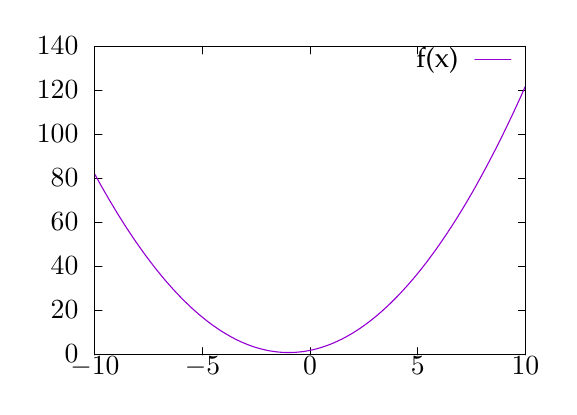
\begin{tikzpicture}[gnuplot,scale=0.5]
%% generated with GNUPLOT 5.2p8 (Lua 5.3; terminal rev. Nov 2018, script rev. 108)
%% Sun 03 Jul 2022 09:26:20 PM CST
\path (0.000,0.000) rectangle (12.500,8.750);
\gpcolor{color=gp lt color border}
\gpsetlinetype{gp lt border}
\gpsetdashtype{gp dt solid}
\gpsetlinewidth{1.00}
\draw[gp path] (1.012,0.616)--(1.192,0.616);
\draw[gp path] (11.947,0.616)--(11.767,0.616);
\node[gp node right] at (0.828,0.616) {$0$};
\draw[gp path] (1.012,1.734)--(1.192,1.734);
\draw[gp path] (11.947,1.734)--(11.767,1.734);
\node[gp node right] at (0.828,1.734) {$20$};
\draw[gp path] (1.012,2.852)--(1.192,2.852);
\draw[gp path] (11.947,2.852)--(11.767,2.852);
\node[gp node right] at (0.828,2.852) {$40$};
\draw[gp path] (1.012,3.970)--(1.192,3.970);
\draw[gp path] (11.947,3.970)--(11.767,3.970);
\node[gp node right] at (0.828,3.970) {$60$};
\draw[gp path] (1.012,5.087)--(1.192,5.087);
\draw[gp path] (11.947,5.087)--(11.767,5.087);
\node[gp node right] at (0.828,5.087) {$80$};
\draw[gp path] (1.012,6.205)--(1.192,6.205);
\draw[gp path] (11.947,6.205)--(11.767,6.205);
\node[gp node right] at (0.828,6.205) {$100$};
\draw[gp path] (1.012,7.323)--(1.192,7.323);
\draw[gp path] (11.947,7.323)--(11.767,7.323);
\node[gp node right] at (0.828,7.323) {$120$};
\draw[gp path] (1.012,8.441)--(1.192,8.441);
\draw[gp path] (11.947,8.441)--(11.767,8.441);
\node[gp node right] at (0.828,8.441) {$140$};
\draw[gp path] (1.012,0.616)--(1.012,0.796);
\draw[gp path] (1.012,8.441)--(1.012,8.261);
\node[gp node center] at (1.012,0.308) {$-10$};
\draw[gp path] (3.746,0.616)--(3.746,0.796);
\draw[gp path] (3.746,8.441)--(3.746,8.261);
\node[gp node center] at (3.746,0.308) {$-5$};
\draw[gp path] (6.480,0.616)--(6.480,0.796);
\draw[gp path] (6.480,8.441)--(6.480,8.261);
\node[gp node center] at (6.480,0.308) {$0$};
\draw[gp path] (9.213,0.616)--(9.213,0.796);
\draw[gp path] (9.213,8.441)--(9.213,8.261);
\node[gp node center] at (9.213,0.308) {$5$};
\draw[gp path] (11.947,0.616)--(11.947,0.796);
\draw[gp path] (11.947,8.441)--(11.947,8.261);
\node[gp node center] at (11.947,0.308) {$10$};
\draw[gp path] (1.012,8.441)--(1.012,0.616)--(11.947,0.616)--(11.947,8.441)--cycle;
\node[gp node right] at (10.479,8.107) {f(x)};
\gpcolor{rgb color={0.580,0.000,0.827}}
\draw[gp path] (10.663,8.107)--(11.579,8.107);
\draw[gp path] (1.012,5.199)--(1.122,4.998)--(1.233,4.802)--(1.343,4.610)--(1.454,4.423)%
  --(1.564,4.240)--(1.675,4.062)--(1.785,3.888)--(1.896,3.719)--(2.006,3.555)--(2.117,3.395)%
  --(2.227,3.240)--(2.337,3.089)--(2.448,2.943)--(2.558,2.801)--(2.669,2.664)--(2.779,2.531)%
  --(2.890,2.403)--(3.000,2.280)--(3.111,2.161)--(3.221,2.047)--(3.332,1.937)--(3.442,1.832)%
  --(3.552,1.731)--(3.663,1.635)--(3.773,1.544)--(3.884,1.457)--(3.994,1.374)--(4.105,1.297)%
  --(4.215,1.223)--(4.326,1.155)--(4.436,1.091)--(4.547,1.031)--(4.657,0.976)--(4.767,0.926)%
  --(4.878,0.880)--(4.988,0.839)--(5.099,0.802)--(5.209,0.770)--(5.320,0.742)--(5.430,0.719)%
  --(5.541,0.701)--(5.651,0.687)--(5.762,0.677)--(5.872,0.673)--(5.982,0.672)--(6.093,0.677)%
  --(6.203,0.686)--(6.314,0.699)--(6.424,0.717)--(6.535,0.740)--(6.645,0.767)--(6.756,0.799)%
  --(6.866,0.835)--(6.977,0.876)--(7.087,0.921)--(7.197,0.971)--(7.308,1.025)--(7.418,1.085)%
  --(7.529,1.148)--(7.639,1.216)--(7.750,1.289)--(7.860,1.366)--(7.971,1.448)--(8.081,1.535)%
  --(8.192,1.626)--(8.302,1.721)--(8.412,1.822)--(8.523,1.926)--(8.633,2.036)--(8.744,2.149)%
  --(8.854,2.268)--(8.965,2.391)--(9.075,2.518)--(9.186,2.650)--(9.296,2.787)--(9.407,2.928)%
  --(9.517,3.074)--(9.627,3.224)--(9.738,3.379)--(9.848,3.539)--(9.959,3.703)--(10.069,3.871)%
  --(10.180,4.044)--(10.290,4.222)--(10.401,4.404)--(10.511,4.591)--(10.622,4.782)--(10.732,4.978)%
  --(10.842,5.179)--(10.953,5.384)--(11.063,5.594)--(11.174,5.808)--(11.284,6.027)--(11.395,6.250)%
  --(11.505,6.478)--(11.616,6.710)--(11.726,6.947)--(11.837,7.189)--(11.947,7.435);
\gpcolor{color=gp lt color border}
\draw[gp path] (1.012,8.441)--(1.012,0.616)--(11.947,0.616)--(11.947,8.441)--cycle;
%% coordinates of the plot area
\gpdefrectangularnode{gp plot 1}{\pgfpoint{1.012cm}{0.616cm}}{\pgfpoint{11.947cm}{8.441cm}}
\end{tikzpicture}
%% gnuplot variables
\label{f::01}
}

\hspace{0.5in}

\subfigure[只有一个解的情况]{
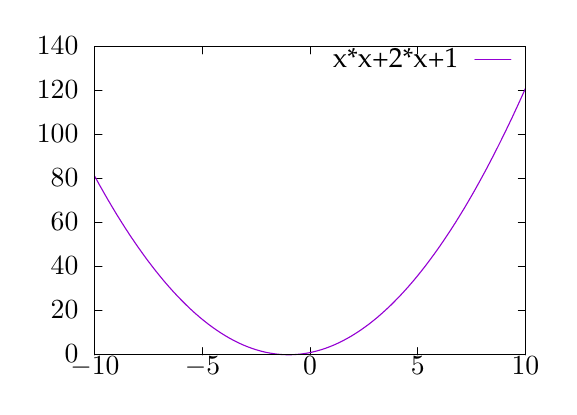
\begin{tikzpicture}[gnuplot,scale=0.5]
%% generated with GNUPLOT 5.2p8 (Lua 5.3; terminal rev. Nov 2018, script rev. 108)
%% Sun 03 Jul 2022 09:06:39 PM CST
\path (0.000,0.000) rectangle (12.500,8.750);
\gpcolor{color=gp lt color border}
\gpsetlinetype{gp lt border}
\gpsetdashtype{gp dt solid}
\gpsetlinewidth{1.00}
\draw[gp path] (1.012,0.616)--(1.192,0.616);
\draw[gp path] (11.947,0.616)--(11.767,0.616);
\node[gp node right] at (0.828,0.616) {$0$};
\draw[gp path] (1.012,1.734)--(1.192,1.734);
\draw[gp path] (11.947,1.734)--(11.767,1.734);
\node[gp node right] at (0.828,1.734) {$20$};
\draw[gp path] (1.012,2.852)--(1.192,2.852);
\draw[gp path] (11.947,2.852)--(11.767,2.852);
\node[gp node right] at (0.828,2.852) {$40$};
\draw[gp path] (1.012,3.970)--(1.192,3.970);
\draw[gp path] (11.947,3.970)--(11.767,3.970);
\node[gp node right] at (0.828,3.970) {$60$};
\draw[gp path] (1.012,5.087)--(1.192,5.087);
\draw[gp path] (11.947,5.087)--(11.767,5.087);
\node[gp node right] at (0.828,5.087) {$80$};
\draw[gp path] (1.012,6.205)--(1.192,6.205);
\draw[gp path] (11.947,6.205)--(11.767,6.205);
\node[gp node right] at (0.828,6.205) {$100$};
\draw[gp path] (1.012,7.323)--(1.192,7.323);
\draw[gp path] (11.947,7.323)--(11.767,7.323);
\node[gp node right] at (0.828,7.323) {$120$};
\draw[gp path] (1.012,8.441)--(1.192,8.441);
\draw[gp path] (11.947,8.441)--(11.767,8.441);
\node[gp node right] at (0.828,8.441) {$140$};
\draw[gp path] (1.012,0.616)--(1.012,0.796);
\draw[gp path] (1.012,8.441)--(1.012,8.261);
\node[gp node center] at (1.012,0.308) {$-10$};
\draw[gp path] (3.746,0.616)--(3.746,0.796);
\draw[gp path] (3.746,8.441)--(3.746,8.261);
\node[gp node center] at (3.746,0.308) {$-5$};
\draw[gp path] (6.480,0.616)--(6.480,0.796);
\draw[gp path] (6.480,8.441)--(6.480,8.261);
\node[gp node center] at (6.480,0.308) {$0$};
\draw[gp path] (9.213,0.616)--(9.213,0.796);
\draw[gp path] (9.213,8.441)--(9.213,8.261);
\node[gp node center] at (9.213,0.308) {$5$};
\draw[gp path] (11.947,0.616)--(11.947,0.796);
\draw[gp path] (11.947,8.441)--(11.947,8.261);
\node[gp node center] at (11.947,0.308) {$10$};
\draw[gp path] (1.012,8.441)--(1.012,0.616)--(11.947,0.616)--(11.947,8.441)--cycle;
\node[gp node right] at (10.479,8.107) {x*x+2*x+1};
\gpcolor{rgb color={0.580,0.000,0.827}}
\draw[gp path] (10.663,8.107)--(11.579,8.107);
\draw[gp path] (1.012,5.143)--(1.122,4.942)--(1.233,4.746)--(1.343,4.554)--(1.454,4.367)%
  --(1.564,4.184)--(1.675,4.006)--(1.785,3.832)--(1.896,3.663)--(2.006,3.499)--(2.117,3.339)%
  --(2.227,3.184)--(2.337,3.033)--(2.448,2.887)--(2.558,2.745)--(2.669,2.608)--(2.779,2.475)%
  --(2.890,2.347)--(3.000,2.224)--(3.111,2.105)--(3.221,1.991)--(3.332,1.881)--(3.442,1.776)%
  --(3.552,1.675)--(3.663,1.579)--(3.773,1.488)--(3.884,1.401)--(3.994,1.319)--(4.105,1.241)%
  --(4.215,1.168)--(4.326,1.099)--(4.436,1.035)--(4.547,0.975)--(4.657,0.920)--(4.767,0.870)%
  --(4.878,0.824)--(4.988,0.783)--(5.099,0.746)--(5.209,0.714)--(5.320,0.686)--(5.430,0.663)%
  --(5.541,0.645)--(5.651,0.631)--(5.762,0.621)--(5.872,0.617)--(5.982,0.616)--(6.093,0.621)%
  --(6.203,0.630)--(6.314,0.643)--(6.424,0.661)--(6.535,0.684)--(6.645,0.711)--(6.756,0.743)%
  --(6.866,0.779)--(6.977,0.820)--(7.087,0.865)--(7.197,0.915)--(7.308,0.970)--(7.418,1.029)%
  --(7.529,1.092)--(7.639,1.161)--(7.750,1.233)--(7.860,1.311)--(7.971,1.392)--(8.081,1.479)%
  --(8.192,1.570)--(8.302,1.666)--(8.412,1.766)--(8.523,1.870)--(8.633,1.980)--(8.744,2.093)%
  --(8.854,2.212)--(8.965,2.335)--(9.075,2.462)--(9.186,2.594)--(9.296,2.731)--(9.407,2.872)%
  --(9.517,3.018)--(9.627,3.168)--(9.738,3.323)--(9.848,3.483)--(9.959,3.647)--(10.069,3.815)%
  --(10.180,3.988)--(10.290,4.166)--(10.401,4.348)--(10.511,4.535)--(10.622,4.727)--(10.732,4.923)%
  --(10.842,5.123)--(10.953,5.328)--(11.063,5.538)--(11.174,5.752)--(11.284,5.971)--(11.395,6.194)%
  --(11.505,6.422)--(11.616,6.654)--(11.726,6.891)--(11.837,7.133)--(11.947,7.379);
\gpcolor{color=gp lt color border}
\draw[gp path] (1.012,8.441)--(1.012,0.616)--(11.947,0.616)--(11.947,8.441)--cycle;
%% coordinates of the plot area
\gpdefrectangularnode{gp plot 1}{\pgfpoint{1.012cm}{0.616cm}}{\pgfpoint{11.947cm}{8.441cm}}
\end{tikzpicture}
%% gnuplot variables
\label{f::02}
}
\hspace{0.5in}
\subfigure[有两个解的情况]{
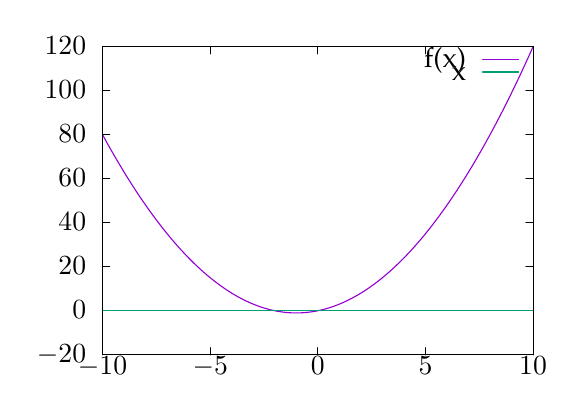
\begin{tikzpicture}[gnuplot,scale=0.5]
%% generated with GNUPLOT 5.2p8 (Lua 5.3; terminal rev. Nov 2018, script rev. 108)
%% Sun 03 Jul 2022 09:19:10 PM CST
\path (0.000,0.000) rectangle (12.500,8.750);
\gpcolor{color=gp lt color border}
\gpsetlinetype{gp lt border}
\gpsetdashtype{gp dt solid}
\gpsetlinewidth{1.00}
\draw[gp path] (1.012,0.616)--(1.192,0.616);
\draw[gp path] (11.947,0.616)--(11.767,0.616);
\node[gp node right] at (0.828,0.616) {$-20$};
\draw[gp path] (1.012,1.734)--(1.192,1.734);
\draw[gp path] (11.947,1.734)--(11.767,1.734);
\node[gp node right] at (0.828,1.734) {$0$};
\draw[gp path] (1.012,2.852)--(1.192,2.852);
\draw[gp path] (11.947,2.852)--(11.767,2.852);
\node[gp node right] at (0.828,2.852) {$20$};
\draw[gp path] (1.012,3.970)--(1.192,3.970);
\draw[gp path] (11.947,3.970)--(11.767,3.970);
\node[gp node right] at (0.828,3.970) {$40$};
\draw[gp path] (1.012,5.087)--(1.192,5.087);
\draw[gp path] (11.947,5.087)--(11.767,5.087);
\node[gp node right] at (0.828,5.087) {$60$};
\draw[gp path] (1.012,6.205)--(1.192,6.205);
\draw[gp path] (11.947,6.205)--(11.767,6.205);
\node[gp node right] at (0.828,6.205) {$80$};
\draw[gp path] (1.012,7.323)--(1.192,7.323);
\draw[gp path] (11.947,7.323)--(11.767,7.323);
\node[gp node right] at (0.828,7.323) {$100$};
\draw[gp path] (1.012,8.441)--(1.192,8.441);
\draw[gp path] (11.947,8.441)--(11.767,8.441);
\node[gp node right] at (0.828,8.441) {$120$};
\draw[gp path] (1.012,0.616)--(1.012,0.796);
\draw[gp path] (1.012,8.441)--(1.012,8.261);
\node[gp node center] at (1.012,0.308) {$-10$};
\draw[gp path] (3.746,0.616)--(3.746,0.796);
\draw[gp path] (3.746,8.441)--(3.746,8.261);
\node[gp node center] at (3.746,0.308) {$-5$};
\draw[gp path] (6.480,0.616)--(6.480,0.796);
\draw[gp path] (6.480,8.441)--(6.480,8.261);
\node[gp node center] at (6.480,0.308) {$0$};
\draw[gp path] (9.213,0.616)--(9.213,0.796);
\draw[gp path] (9.213,8.441)--(9.213,8.261);
\node[gp node center] at (9.213,0.308) {$5$};
\draw[gp path] (11.947,0.616)--(11.947,0.796);
\draw[gp path] (11.947,8.441)--(11.947,8.261);
\node[gp node center] at (11.947,0.308) {$10$};
\draw[gp path] (1.012,8.441)--(1.012,0.616)--(11.947,0.616)--(11.947,8.441)--cycle;
\node[gp node right] at (10.479,8.107) {f(x)};
\gpcolor{rgb color={0.580,0.000,0.827}}
\draw[gp path] (10.663,8.107)--(11.579,8.107);
\draw[gp path] (1.012,6.205)--(1.122,6.004)--(1.233,5.808)--(1.343,5.616)--(1.454,5.429)%
  --(1.564,5.246)--(1.675,5.068)--(1.785,4.894)--(1.896,4.725)--(2.006,4.561)--(2.117,4.401)%
  --(2.227,4.246)--(2.337,4.095)--(2.448,3.949)--(2.558,3.807)--(2.669,3.670)--(2.779,3.537)%
  --(2.890,3.409)--(3.000,3.286)--(3.111,3.167)--(3.221,3.053)--(3.332,2.943)--(3.442,2.838)%
  --(3.552,2.737)--(3.663,2.641)--(3.773,2.550)--(3.884,2.463)--(3.994,2.381)--(4.105,2.303)%
  --(4.215,2.230)--(4.326,2.161)--(4.436,2.097)--(4.547,2.037)--(4.657,1.982)--(4.767,1.932)%
  --(4.878,1.886)--(4.988,1.845)--(5.099,1.808)--(5.209,1.776)--(5.320,1.748)--(5.430,1.725)%
  --(5.541,1.707)--(5.651,1.693)--(5.762,1.683)--(5.872,1.679)--(5.982,1.678)--(6.093,1.683)%
  --(6.203,1.692)--(6.314,1.705)--(6.424,1.723)--(6.535,1.746)--(6.645,1.773)--(6.756,1.805)%
  --(6.866,1.841)--(6.977,1.882)--(7.087,1.927)--(7.197,1.977)--(7.308,2.032)--(7.418,2.091)%
  --(7.529,2.154)--(7.639,2.222)--(7.750,2.295)--(7.860,2.373)--(7.971,2.454)--(8.081,2.541)%
  --(8.192,2.632)--(8.302,2.728)--(8.412,2.828)--(8.523,2.932)--(8.633,3.042)--(8.744,3.155)%
  --(8.854,3.274)--(8.965,3.397)--(9.075,3.524)--(9.186,3.656)--(9.296,3.793)--(9.407,3.934)%
  --(9.517,4.080)--(9.627,4.230)--(9.738,4.385)--(9.848,4.545)--(9.959,4.709)--(10.069,4.877)%
  --(10.180,5.050)--(10.290,5.228)--(10.401,5.410)--(10.511,5.597)--(10.622,5.789)--(10.732,5.984)%
  --(10.842,6.185)--(10.953,6.390)--(11.063,6.600)--(11.174,6.814)--(11.284,7.033)--(11.395,7.256)%
  --(11.505,7.484)--(11.616,7.716)--(11.726,7.953)--(11.837,8.195)--(11.947,8.441);
\gpcolor{color=gp lt color border}
\node[gp node right] at (10.479,7.799) {x};
\gpcolor{rgb color={0.000,0.620,0.451}}
\draw[gp path] (10.663,7.799)--(11.579,7.799);
\draw[gp path] (1.012,1.734)--(1.122,1.734)--(1.233,1.734)--(1.343,1.734)--(1.454,1.734)%
  --(1.564,1.734)--(1.675,1.734)--(1.785,1.734)--(1.896,1.734)--(2.006,1.734)--(2.117,1.734)%
  --(2.227,1.734)--(2.337,1.734)--(2.448,1.734)--(2.558,1.734)--(2.669,1.734)--(2.779,1.734)%
  --(2.890,1.734)--(3.000,1.734)--(3.111,1.734)--(3.221,1.734)--(3.332,1.734)--(3.442,1.734)%
  --(3.552,1.734)--(3.663,1.734)--(3.773,1.734)--(3.884,1.734)--(3.994,1.734)--(4.105,1.734)%
  --(4.215,1.734)--(4.326,1.734)--(4.436,1.734)--(4.547,1.734)--(4.657,1.734)--(4.767,1.734)%
  --(4.878,1.734)--(4.988,1.734)--(5.099,1.734)--(5.209,1.734)--(5.320,1.734)--(5.430,1.734)%
  --(5.541,1.734)--(5.651,1.734)--(5.762,1.734)--(5.872,1.734)--(5.982,1.734)--(6.093,1.734)%
  --(6.203,1.734)--(6.314,1.734)--(6.424,1.734)--(6.535,1.734)--(6.645,1.734)--(6.756,1.734)%
  --(6.866,1.734)--(6.977,1.734)--(7.087,1.734)--(7.197,1.734)--(7.308,1.734)--(7.418,1.734)%
  --(7.529,1.734)--(7.639,1.734)--(7.750,1.734)--(7.860,1.734)--(7.971,1.734)--(8.081,1.734)%
  --(8.192,1.734)--(8.302,1.734)--(8.412,1.734)--(8.523,1.734)--(8.633,1.734)--(8.744,1.734)%
  --(8.854,1.734)--(8.965,1.734)--(9.075,1.734)--(9.186,1.734)--(9.296,1.734)--(9.407,1.734)%
  --(9.517,1.734)--(9.627,1.734)--(9.738,1.734)--(9.848,1.734)--(9.959,1.734)--(10.069,1.734)%
  --(10.180,1.734)--(10.290,1.734)--(10.401,1.734)--(10.511,1.734)--(10.622,1.734)--(10.732,1.734)%
  --(10.842,1.734)--(10.953,1.734)--(11.063,1.734)--(11.174,1.734)--(11.284,1.734)--(11.395,1.734)%
  --(11.505,1.734)--(11.616,1.734)--(11.726,1.734)--(11.837,1.734)--(11.947,1.734);
\gpcolor{color=gp lt color border}
\draw[gp path] (1.012,8.441)--(1.012,0.616)--(11.947,0.616)--(11.947,8.441)--cycle;
%% coordinates of the plot area
\gpdefrectangularnode{gp plot 1}{\pgfpoint{1.012cm}{0.616cm}}{\pgfpoint{11.947cm}{8.441cm}}
\end{tikzpicture}
%% gnuplot variables
\label{f::03}
}
\caption{三种不同的解的情况}
\end{figure}

\section{求解过程}

\thispagestyle{empty}
% 流程图定义基本形状
\tikzstyle{startstop} = [rectangle, rounded corners, minimum width = 2cm, minimum height=1cm,text centered, draw = black]
\tikzstyle{io} = [trapezium, trapezium left angle=70, trapezium right angle=110, minimum width=2cm, minimum height=1cm, text centered, draw=black]
\tikzstyle{process} = [rectangle, minimum width=3cm, minimum height=1cm, text centered, draw=black]
\tikzstyle{decision} = [diamond, aspect = 3, text centered, draw=black]
% 箭头形式
\tikzstyle{arrow} = [->,>=stealth]
\begin{tikzpicture}[node distance=1cm]

%定义流程图具体形状
\node[startstop](start){Start};
\node[io, below of = start, yshift = -1cm](in1){输入方程};
\node[decision, below of = in1, yshift = -1cm](dec1){是否选择公式法 ?};
\node[decision, below of = dec1,xshift = -4cm, yshift = -1cm](dec2){$\triangle \geq or \ge 0$ ?};
\node[process, below of = dec2, xshift = 4cm, yshift = -1cm](pro1){运用公式得出解};
\node[decision, right of = dec1, xshift = 5.5cm](dec3){是否为$(x+a)^2=b$的形式 ?};
\node[process, below of = dec3, xshift = -4cm,yshift = -1cm](pro2){运用方法一的结论得出解};
\node[process, right of = pro2, xshift = 4cm](pro3){运用配方法的结论得出解};
\node[io, below of = pro1, yshift = -1cm](out1){输出解的值或方程无解};
\node[startstop, below of = out1, yshift = -1cm](stop){Stop};
\coordinate (point1) at (-3cm, -3cm);
%连接具体形状
\draw [arrow] (start) -- (in1);
\draw [arrow] (in1) -- (dec1);
\draw [arrow] (dec1) -- node [right] {yes} (dec2);
\draw [arrow] (dec1) -- node [above] {no} (dec3);
\draw [arrow] (dec2) -- node [right] {yes} (pro1);
\draw [arrow] (dec2) -- node [above] {no} (out1);
\draw [arrow] (dec3) -- node [right] {yes} (pro2);
\draw [arrow] (dec3) -- node [left] {no} (pro3);
\draw [arrow] (pro1) -- (out1);
\draw [arrow] (pro2) -- (out1);
\draw [arrow] (pro3) -- (out1);
\draw [arrow] (out1) -- (stop);
\end{tikzpicture}

\end{document}
